\documentclass[11pt,a4paper]{book}
\textwidth 170 mm
\textheight 250 mm
\topmargin -15 mm
\oddsidemargin -5 mm
\evensidemargin -5 mm

\newcounter{ProblemNo}
\setcounter{ProblemNo}{0}
\def\tempID{0}
%\def\UndAns{} %% <-------------- Uncomment in final version!!
\def\UndAns{\underline}
\def\UndAns{\underline}
\newcommand{\ZOdg}[1]{}
\def\text{}
%\def\dfrac{\displaystyle\frac}

\usepackage{amsfonts,amssymb,amsmath}
\usepackage{graphicx}
\DeclareGraphicsExtensions{.pdf,.PDF,.png,.PNG} % prefer pdf to png
\usepackage{etoolbox}
\usepackage{sidepicture}
\newcommand{\problemID}[3]{\def\tempID{#1 (#3)}\ignorespacesafterend}
%\newcommand{\problemID}[3]{\def\tempID{#1}\noindent{\bf #1, #2}\par}
%\newcommand{\problemID}[3]{\def\tempID{#3: \##1}\par}
%\newcommand{\problemRating}[3]{{\bf #1, #2, #3}\par}
%\newcommand{\problemID}[3]{\def\tempID{\# #1}\par}
%\newcommand{\problemRating}[3]{}
%\newcommand{\xProblem}[8]{#1\par (A) #2\quad (B) #3\quad  (C) #4\quad  (D) #5\quad (E) #6\par Correct: #7\bigskip\bigskip\par }

%\usepackage{xcolor}
%\usepackage{everypage}
%\usepackage[absolute]{textpos}
%\usepackage{rotating}
%\AddEverypageHook{\begin{textblock*}{2.5cm}(0.7cm,5cm)\begin{turn}{90}{\color{red}\Huge\sc Solutions included - do not use for contest}\end{turn}\end{textblock*}}

\newcommand{\Problem}[9]
{%\newpage
%\noindent\addtocounter{ProblemNo}{1}{\bf\arabic{ProblemNo}.\hspace{3pt}~}%
\noindent\addtocounter{ProblemNo}{1}{\bf\tempID.\hspace{3pt}~}%
\edef\answer{{#7}}\def\SettingMode{#8}%
\def\VLine{\vrule height14pt width0pt\quad}#1\nopagebreak\vspace{1ex}\newline%
\VLine\expandafter\ifstrequal\answer{A}{\UndAns{(\rlap{\bf A}\phantom{\bf C})}\ZOdg{A}}{(\rlap{\bf A}\phantom{\bf C})}\nolinebreak\hspace{3pt}%
\ifnum\SettingMode=3{#2}\else\rlap{#2}\fi\quad\ifnum\SettingMode=3\newline\VLine\else\hfil\fi%
\expandafter\ifstrequal\answer{B}{\UndAns{(\rlap{\bf B}\phantom{\bf C})}\ZOdg{B}}{(\rlap{\bf B}\phantom{\bf C})}\nolinebreak\hspace{3pt}%
\ifnum\SettingMode=3{#3}\else\rlap{#3}\fi\quad\ifnum\SettingMode=2\newline\VLine\else\ifnum\SettingMode=3\newline\VLine\else\ifnum\SettingMode=6{\phantom{({\bf C})}\quad\hspace{6pt}\hfil\hfil\newline\VLine}\else\hfil\fi\fi\fi%
\expandafter\ifstrequal\answer{C}{\UndAns{(\rlap{\bf C}\phantom{\bf C})}\ZOdg{C}}{({\bf C})}\nolinebreak\hspace{3pt}%
\ifnum\SettingMode=3{#4}\else\rlap{#4}\fi\quad\ifodd\SettingMode\newline\VLine\else\hfil\fi%
\expandafter\ifstrequal\answer{D}{\UndAns{(\rlap{\bf D}\phantom{\bf C})}\ZOdg{D}}{(\rlap{\bf D}\phantom{\bf C})}\nolinebreak\hspace{3pt}%
\ifnum\SettingMode=3{#5}\else\rlap{#5}\fi\quad\ifnum\SettingMode>1\ifnum\SettingMode<6\newline\VLine\else\hfil\fi\else\hfil\fi%
\expandafter\ifstrequal\answer{E}{\UndAns{(\rlap{\bf E}\phantom{\bf C})}\ZOdg{E}}{(\rlap{\bf E}\phantom{\bf C})}\nolinebreak\hspace{3pt}%
\ifnum\SettingMode=3{#6}\else\rlap{#6}\fi\quad\ifnum\SettingMode=1\hfil\phantom{({\bf C})}\fi\hspace{3pt}\hfil\par\vspace{2ex}\par\noindent{\sc Solution: }#9\bigskip}


\def\TheHead{Ecolier Finalized}
\makeatletter
\def\ps@pKSF{
\def\@oddfoot{\hfill{\rm \thepage}\hfill}\def\@evenfoot{\hfill{\rm \thepage}\hfill}
\def\@oddhead{\hfill{\em \TheHead}\hfill}\def\@evenhead{\hfill{\em \TheHead}\hfill}
}
\makeatother 
\pagestyle{pKSF}

\begin{document}

\noindent{\large\bf Ecolier}\bigskip

\noindent\fbox{3 points}\bigskip

\problemID{1}{20173}{Switzerland}%
\problemRating{E}{3}{G}%
\Problem{Which square is cut into 2 different shapes?}
{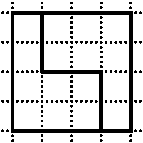
\includegraphics{E01-1}}{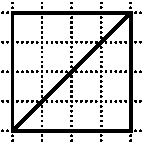
\includegraphics{E01-2}}{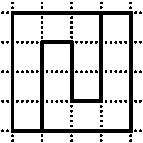
\includegraphics{E01-3} }{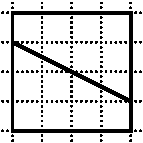
\includegraphics{E01-4}}{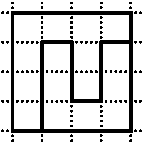
\includegraphics{E01-5}}
{E}{0}
{The shapes in the figure (colored in gray and white) are different. The gray shape is made from 9 squares, and white shape is made from 7 squares.

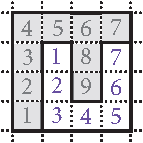
\includegraphics[scale=1.0]{E01-6}}

\problemID{2}{20174}{Denmark}%
\problemRating{E}{3}{L}%
\Problem{What is the smallest number of ladders the firefighter must use to reach the fire without jumping?\newline
\includegraphics{E02-1}}
{4}{5}{6}{7}{8}
{C}{0}
{The firefighter must reach the fire using only stairs and without jumping. The minimum number of ladders required for this is 6. See the figure.
\newline
\includegraphics{E02-2}}

\problemID{3}{20175}{Russia}%
\problemRating{E}{3}{G}%
\Problem{The table consists of 28 white cells: \newline
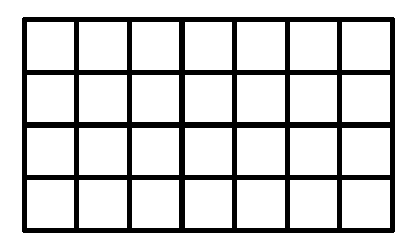
\includegraphics[scale=0.7]{E03-1} \newline
Ira paints 2 rows and 1 column. \newline
A row is from left to right.  \newline
A column is from top to bottom.  \newline
How many cells will remain white?}
{8}{10}{12}{14}{17}
{C}{0}
{If we color two rows with green and one column with yellow, the total number of remaining white cells will be 12. 
\newline
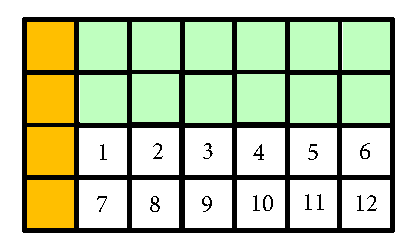
\includegraphics[scale=0.7]{E03-2}}

\NSidePictureEPS[scale=0.85]{E04-2}{\problemID{4}{20176}{Ghana}%
\problemRating{E}{3}{G}%
\Problem{Soccer players numbered 1 to 11 stand in a circle. \newline
Each player kicks the ball to the third player on their left. \newline
Player 1 starts. \newline
This kicking pattern continues until a player \textbf{has} the ball for the second time. \newline
What is the number of the player who \textbf{kicked} the ball last?}
{7}{8}{9}{10}{11}
{C}{1}
{The 4th pass will be from the player wearing shirt number 10 to the player wearing shirt number 2.
\newline
The 7th pass will be from the player wearing shirt number 8 to the player wearing shirt number 11.
\newline
The 10th pass will be from the player wearing shirt number 6 to the player wearing shirt number 9.
\newline
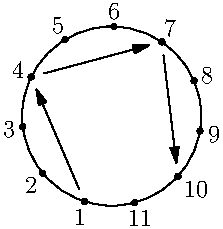
\includegraphics[scale=0.85]{E04-1}}}

\problemID{5}{20177}{Iran}%
\problemRating{E}{3}{N}%
\Problem{Mohammad wrote 3 consecutive 4-digit numbers in a row. \newline
His sister erased some digits. \newline
What are the missing digits (from left to right)? \newline
(For example, 213, 214, 215 are 3 consecutive 3-digit numbers.) \newline

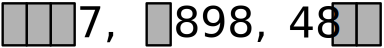
\includegraphics{E05-1}}
{389, 3, 99}{489, 3, 96}{489, 4, 98}{489, 4, 99}{488, 4, 99}
{D}{0}
{The consecutive numbers are: \newline
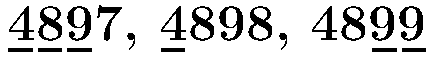
\includegraphics{E05-2}
\newline
The missing digits are: 489, 4, 99}

\problemID{6}{20178}{Nigeria}%
\problemRating{E}{3}{N}%
\Problem{Lizzy pays 7 dollars for 3 items. \newline
The cost of each item is different and is a whole number.  \newline
How much is the most expensive item?}
{2 dollars}{3 dollars}{4 dollars}{5 dollars}{6 dollars}
{C}{0}
{Since the cost of each item is a whole number of dollars and the total cost is 7 dollars, the possible costs of the items are 1 dollar, 2 dollars, 4 dollars. Therefore, the most expensive item could cost 4 dollars.}

\problemID{7}{20179}{Poland}%
\problemRating{E}{3}{G}%
\Problem{A cat knocks off 1 block from Felix's construction.
\newline
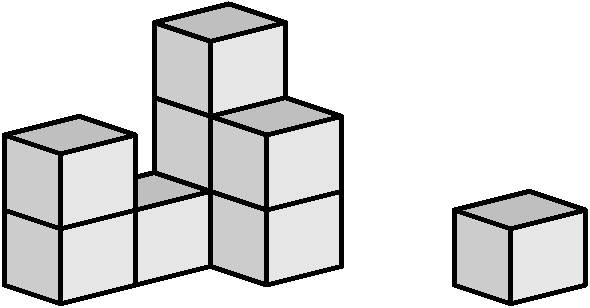
\includegraphics[scale=0.5]{E07-1}
\newline
What could this construction have looked like \textbf{before} the block was knocked off?}
{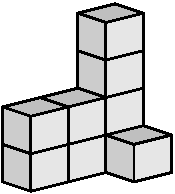
\includegraphics{E07-2}}{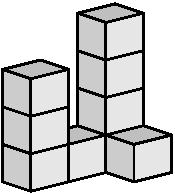
\includegraphics{E07-3}}{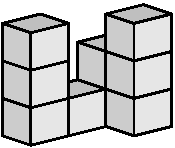
\includegraphics{E07-4}}{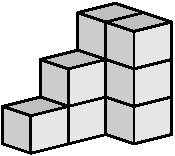
\includegraphics{E07-5}}{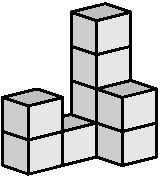
\includegraphics{E07-6}}
{E}{1}
{A cat knocked off one block. When we look Felix's construction, we see that the constructions in options A, B, C, and D differ by two or more blocks from his construction now. Only answer E differs by only one block.}

\problemID{8}{20180}{Iraq}%
\problemRating{E}{3}{L}%
\Problem{Alex has a Kangaroo poster on the kitchen wall. 
\newline
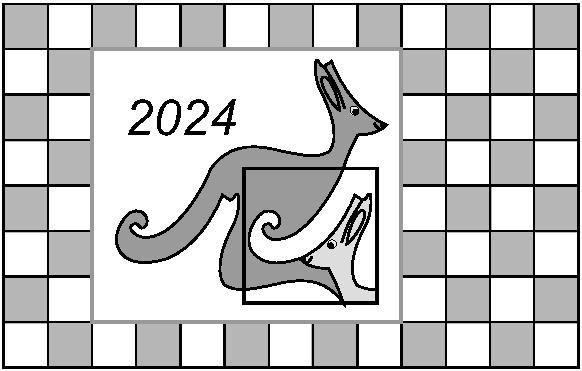
\includegraphics[scale=0.8]{E08-1}
\newline
How many grey tiles are there behind the poster?}
{15}{21}{25}{30}{35}
{B}{0}
{If we remove the poster, we would be able to see all the 21 gray tiles that are behind the poster, see the picture. 
\newline
Alternatively, if we begin from the top of the poster, we can notice 3 gray tiles in the first row, 4 will be in the next, 3 in the following, 4 again, and so on. We have a total of 6 rows behind the poster, with a repeating pattern of 3 tiles in one row and 4 tiles in the second row. This results in total of 7 tiles for every 2 rows, or 21 tiles for all 6 rows.
\newline
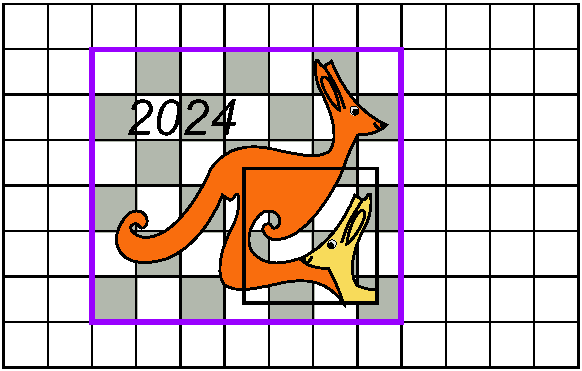
\includegraphics[scale=0.8]{E08-2}}

\noindent\fbox{4 points}\bigskip

\problemID{9}{20181}{Costa Rica}%
\problemRating{E}{4}{N}%
\Problem{Antonia and Lucian toss a coin.

\begin{center}
\includegraphics{E09-1}
\end{center}

If the child sees the purple side, the child advances 3 steps. \newline
If the child sees the green side, the child goes back 1 step or stays at the starting position. \newline
Both started in front of number 1 and each tossed the coin 4 times. 
\newline
Antonia advanced to number 4 and Lucian advanced to number 8. \newline
How many times in total did they see the green side of the coin?}
{1}{2}{3}{4}{5}
{C}{0}
{Antonia advanced to number 4 meaning that he must have seen 2 purple sides and 2 green sides: $3+3-1-1=4$. 
Lucian advanced to number 8 meaning that she must have seen 3 purple sides and 1 green side: $3+3+3-1=8$. 
In total, they have seen the green side 3 times.}

\problemID{10}{20182}{Switzerland}%
\problemRating{E}{4}{L}%
\Problem{There are five different kinds of fruit in a bowl:

\includegraphics{E10-1} 
\includegraphics{E10-2} 
\includegraphics{E10-3} 
\includegraphics{E10-4} 
\includegraphics{E10-5}.\newline
Ann likes 
\includegraphics{E10-3}.
\newline
Ben likes 
\includegraphics{E10-1} 
\includegraphics{E10-2} 
\includegraphics{E10-3} 
\includegraphics{E10-4} 
\includegraphics{E10-5}.\newline
Cam likes 
\includegraphics{E10-3} 
\includegraphics{E10-4} 
\includegraphics{E10-5}.
\newline
Dan likes 
\includegraphics{E10-3} 
\includegraphics{E10-5}.
\newline
Eli likes 
\includegraphics{E10-2} 
\includegraphics{E10-4}.
\newline
Everyone gets a fruit they like.
\newline
Everyone gets a different kind of fruit. 
\newline
What does Ben get?}
{
\includegraphics{E10-1}}{
\includegraphics{E10-2}}{
\includegraphics{E10-3}}{
\includegraphics{E10-4}}{
\includegraphics{E10-5}}
{A}{0}
{Ann gets  
\includegraphics{E10-3} because this is the only fruit she likes.
\newline
Dan gets 
\includegraphics{E10-5} because Ann gets the other fruit he likes.
\newline
Cam gets 
\includegraphics{E10-4} because Ann and Dan get the other fruits he likes. 
\newline
Eli gets 
\includegraphics{E10-2} because Cam got the other fruit she likes.
\newline
Ben must have got 
\includegraphics{E10-1} because this is the only fruit no one else likes.
\newline
Solution 2: 
Note that we could observe that the apple is the only fruit on the list of liked fruits. Only Ben likes apple of all fruits. Hence, the answer is that Ben gets the apple.}

\NSidePictureEPS{E11-6}{\problemID{11}{20183}{Poland}%
\problemRating{E}{4}{L}%
\Problem{Ada has built a tower of 8 discs, as in the picture. \newline
Ada removes the second disc from the bottom of this tower. \newline
Then she removes the third disc from the bottom of the new tower. \newline
Then she removes the fourth disc from the bottom of the new tower.
Then she removes the fifth disc from the bottom of the new tower. \newline
Which tower does Ada end up with?}
{\includegraphics{E11-1}}{\includegraphics{E11-2}}{\includegraphics{E11-3}}{\includegraphics{E11-4}}{\includegraphics{E11-5}}
{B}{0}
{b/w version: \includegraphics{E11-7}
\includegraphics{E11-8} \includegraphics{E11-9} \includegraphics{E11-10} \includegraphics{E11-11} \includegraphics{E11-12}\newline
Let us use the initial letters of the colors to represent the disks on the tower starting from the bottom. We have, \newline
O\newline
B\newline
O\newline
W\newline
B\newline
O\newline
W\newline
B \newline
First, remove the 2nd disk or colored W from the bottom, what is left is BOBWOBO.\newline
Next remove the 3rd disk or colored B from the new tower. What is left is BOWOBO.\newline
Now remove the 4th disk which is O, what is left is BOWBO.\newline
Lastly remove the 5th disk or colored O, what is left is BOWB or \newline
Blue, Orange, White, Blue.\newline\newline
Solution 2: \newline
1. Ada removes the second (lower white) disk from the bottom of this tower. \newline
2. Then she removes the third (middle blue) disk from the bottom of the new tower. \newline
3. Then she removes the fourth (middle orange) disk of the new tower and then the fifth (top orange) disk of the new tower. \newline
The tower Ada ends up with is \includegraphics{E11-2}}}

\NSidePictureEPS[scale=0.2]{E12-1}{\problemID{12}{20184}{United Kingdom}%
\problemRating{E}{4}{L}%
\Problem{Peter the penguin goes fishing every day and brings back 9 fish for his 2 chicks.\newline
Each day, he gives 5 fish to the first chick he sees and 4 fish to the second chick, which they eat.\newline
Over the last few days, 1 chick has eaten 26 fish.\newline
How many fish has the other chick eaten?}
{19}{22}{25}{28}{31}
{D}{0}
{To have eaten 26 fish, the first chick must have eaten 4 fish four times and 5 fish twice.  Therefore the second chick must have eaten 5 fish four times and 4 fish twice.  Hence the number of fish the second chick ate was $5\times 4 + 4\times 2 = 28$.}}

\problemID{13}{20185}{China}%
\problemRating{E}{4}{A}%
\Problem{7 cards, numbered 1 to 7, are placed in 4 overlapping rings. \newline
The sum of the numbers in each ring is 10. \newline
Which number is under the question mark?\newline\includegraphics{E13-1}}
{1}{2}{4}{5}{7}
{A}{0}
{The number on the right of 6 must be 4 for the sum in the first ring to be 10. The number on the left of 3 must be 7  for the sum in the last ring to be 10. The sum of the number under the question mark and the one to the left of it must be 6, and sum of the number under the question mark and the one to the right of it must be 3. The numbers in these three cards have to be 1, 2, and 5, meaning that 1 is common in these sum, i.e. under the question mark: $1+2=3$ and $1+5=6$.\newline
\includegraphics{E13-2}}

\problemID{14}{20186}{Germany}%
\problemRating{E}{4}{L}%
\Problem{\includegraphics{E14-3}\newline
Lucas wants to make a caterpillar that has a head, a tail and either 1, 2 or 3 puzzle pieces in between. \newline
How many different caterpillars can Lucas make without flipping pieces?}
{3}{4}{5}{6}{7}
{B}{0}
{coloured version: \includegraphics{E14-4}\newline
\includegraphics{E14-2}}

\NSidePictureEPS{E15-2}{\problemID{15}{20187}{Brazil}%
\problemRating{E}{4}{N}%
\Problem{John writes the numbers 1 to 4 on a sheet. \newline
Then he flips the sheet and writes the numbers 5 to 8, as shown. \newline
After that, he cuts the sheet into 4 rectangular cards and puts them in a row:\newline
\includegraphics{E15-1}\newline
What is the sum of the numbers represented by the question marks?}
{3}{4}{5}{6}{7}
{B}{0}
{From the figure with the sheet, we can see that 6 is behind 2, 7 behind 1, 8 behind 3, 5 behind 4. The numbers under the ? marks are behind 7 and 8, namely 1 and 3 with a sum 4.
\newline\newline
Solution 2: \newline
The numbers on the flipping sheet are as follows:\newline
1 is matched with 7.  \newline
2 is matched with 6.  \newline 
4 is matched with 5. \newline
3 is matched with 8. \newline
\newline
When we put these numbers in a row, we notice that there are two missing numbers, which we'll show with question marks 7 and 8. Their corresponding behind numbers are 1 and 3. So, if we add 1 and 3 together, we get 4.}}

\problemID{16}{20188}{Finland}%
\problemRating{E}{4}{G}%
\Problem{A floor is covered with 2 kinds of tile \includegraphics{E16-1} and \includegraphics{E16-2}.
\newline
The rectangles have size $23\ \textup{cm} \times 11\ \textup{cm}$.
\newline
The picture shows a part of the floor.
\newline
What is the side-length of the square tiles? 
\newline
\includegraphics{E16-3}}
{$3\ \textup{cm}$}{$4\ \textup{cm}$}{$5\ \textup{cm}$}{$6\ \textup{cm}$}{$7\ \textup{cm}$}
{D}{0}
{coloured version: \includegraphics{E16-4} \includegraphics{E16-5} \includegraphics{E16-6}
\newline
The long side of the tile equals the short side of the tile and two sides of the square. Thus, two sides of the square equal $23-11=12$ cm, and one side of the square equals $12\div 2=6$ cm.}

\noindent\fbox{5 points}\bigskip

\problemID{17}{20189}{Greece}%
\problemRating{E}{5}{N}%
\Problem{A student has 3 cards with numbers on them.\newline
Their sum is 782.\newline
Unfortunately, a worm ate part of each card.\newline
What is the sum of the 3 missing digits?\newline
\includegraphics{E17-1}}
{8}{9}{10}{11}{12}
{D}{0}
{The missing number in the units is $5$ so that $3+4+5= 12$ (which means $2$ and $1$ to carry). The tens digits (with the carry) must add up to $8$, so without the carry it is $7$. A $1$ is already present, so the other two (the missing ones) must add to $6$ . Any combination of digits that add up to $6$ would do. So the missing numbers add up to $6+5 = 11$. Note there are many examples of numbers that satisfy the conditions, for as long as the two missing tens digits add up to $6$.
Examples: $213+154+415 = 782$ or $223+144+415 = 782$ or $233+134+415 = 782$, etc.}

\problemID{18}{20190}{Catalonia}%
\problemRating{E}{5}{A}%
\Problem{Lucy weighs some blocks.\newline 
\includegraphics{E18-1}\newline
How much do the 3 different blocks weigh together?}
{$270\ \textup{g}$}{$280\ \textup{g}$}{$290\ \textup{g}$}{$300\ \textup{g}$}{$310\ \textup{g}$}
{A}{0}
{If you add the 3 scales then you will have every block 2 times. 
$(200\ \textup{g} + 100\ \textup{g} + 240\ \textup{g}) : 2 = 540\ \textup{g} : 2=270\ \textup{g}$}

\problemID{19}{20191}{Slovakia}%
\problemRating{E}{5}{N}%
\Problem{There are 60 pupils on a trip. \newline
When they line up, the colours of their reflective vests follow the pattern: yellow, green, yellow, green... \newline
The colours of their backpacks follow a different pattern: red, brown, orange, red, brown, orange... \newline
How many pupils with a yellow reflective vest also have an orange backpack?}
{3}{4}{6}{8}{10}
{E}{0}
{YR, GB, YO, GR, YB, GO, YR, GB, YO .... oh you notice that the pattern started to repeat itself after 6 pupils. Now we can see that there will be one YO (Yellow/Orange) for each 6 and we need to have the pattern 10 times. $1 \times 10 = 10$ pupils with yellow vest and orange backback.}

\problemID{20}{20192}{Poland}%
\problemRating{E}{5}{N}%
\Problem{In the following calculations, the same digits are hidden under the same figures. \newline
Different digits are hidden under different figures.
\newline
\includegraphics{E20-1}
\newline
What is the value of \includegraphics{E20-2} ?}
{\(0\)}{\(15\)}{\(18\)}{\(28\)}{\(30\)}
{D}{0}
{$7+7=14$, $4+7=11$, $7\cdot4\cdot1=28$.}

\newpage\problemID{21}{20193}{Republic of China (Taiwan)}%
\problemRating{E}{5}{L}%
\Problem{There are exactly 2 frogs in each row and each column. \newline
The frogs decide that 2 of them will jump to a neighbouring empty cell at the same time. \newline
Neighbouring cells have a side in common. \newline
After that, there still are exactly 2 frogs in each row and in each column. \newline
In how many ways can the frogs do this? \newline
\includegraphics{E21-1}}
{1}{2}{3}{4}{5}
{D}{0}
{(D) 4

\includegraphics{E21-2}

The frogs can do this in 4 ways, as shown below: 
\newline 
\includegraphics{E21-1}
\newline\newline
\includegraphics{E21-3} \quad \includegraphics{E21-4} \quad \includegraphics{E21-5} \quad \includegraphics{E21-6}}

\problemID{22}{20194}{Turkey}%
\problemRating{E}{5}{L}%
\Problem{The figure below shows a beehive with 9 cells. \newline
There is honey in some cells. \newline
The number in each cell shows how many neighbouring cells contain honey.
Neighbouring cells have a side in common. \newline
How many cells contain honey?\newline
\includegraphics{E22-1}}
{4}{5}{6}{7}{8}
{C}{0}
{\includegraphics{E22-2}}

\problemID{23}{20195}{Poland}%
\problemRating{E}{5}{L}%
\Problem{3 girls go to the tray one after the other and take some cookies.
\newline
\includegraphics{E23-1} \newline
One of the girls takes all the hearts available on the tray. \newline
Another girl takes all the white cookies available on the tray. \newline
Another girl takes all the large cookies available on the tray. \newline
However, they do not necessarily take the cookies in this order. \newline

One girl takes $3$ cookies, one takes $6$ cookies and one takes $7$ cookies. \newline
Which of the following  sets of cookies does one of these girls take?}
{\includegraphics{E23-2}
    \includegraphics{E23-2}
        \includegraphics{E23-3}}{\includegraphics{E23-4}
    \includegraphics{E23-5}
        \includegraphics{E23-5}
            \includegraphics{E23-5}
                \includegraphics{E23-2}
                    \includegraphics{E23-2}
                        \includegraphics{E23-3}}{\includegraphics{E23-5}
    \includegraphics{E23-5}
        \includegraphics{E23-5}
            \includegraphics{E23-2}
                \includegraphics{E23-2}
                        \includegraphics{E23-3}}{\includegraphics{E23-6}
    \includegraphics{E23-6}
        \includegraphics{E23-6}
            \includegraphics{E23-6}
                \includegraphics{E23-3}
                    \includegraphics{E23-4}}{\includegraphics{E23-5}
                    \includegraphics{E23-5}
                        \includegraphics{E23-5}}
{E}{1}
{The first girl did not take the hearts (there were $11$ of them). If she took the white cookies, there would be $9$ hearts left: $4$ large and $5$ small ones, and the conditions of the problem would not be fulfilled. So the first girl took $7$ large cookies, the second took $6$ small hearts, and the third took $3$ small round white cookies.}

\problemID{24}{20196}{Russia}%
\problemRating{E}{5}{G}%
\Problem{There are 2 types of blocks: white \includegraphics[scale=0.3]{E24-1} and red \includegraphics[scale=0.3]{E24-2}. \newline
A small cube can be made of 4 white blocks or of 1 white and 1 red block. \newline
The large cube shown in the picture is made of small cubes. \newline
What is the smallest number of white blocks needed to make the large cube?  \newline
\includegraphics[scale=0.3]{E24-3}}
{8}{11}{13}{14}{23}
{D}{0}
{This cube consists of 8 simple cubes. Every simple cube contains at least 1 white element. Two simple cubes of shown cube consist of 4 white elements. Therefore the smallest number of white elements is $6 + 4 + 4 = 14$.}


\end{document}